\documentclass{article}

\usepackage[left=1.5cm, right=1.5cm, top=3cm, bottom = 3cm]{geometry}

\usepackage{amsmath}
\usepackage{amsfonts}
\usepackage{amssymb}
\usepackage{graphicx}
\usepackage{float}
\usepackage{indentfirst}
\usepackage{wrapfig}
\usepackage{latexsym}
\usepackage{hyperref}
\usepackage{feynmf}
\linespread{1.1}

\author{SM-at-THU}
\title{\bf{Solutions to Pathria's Statistical Mechanics}\\Chapter 2}

\begin{document}
\maketitle
\section*{Problem 2.1}

\section*{Problem 2.2}

\section*{Problem 2.3}
The Hamiltonian of the rotator is a function of the angular momentum $L$. 
$$
H = f(L)
$$
Now we divide the phase space into cells with volume $h$ by lines with constant energies:
\begin{figure}[!htp]
\centering
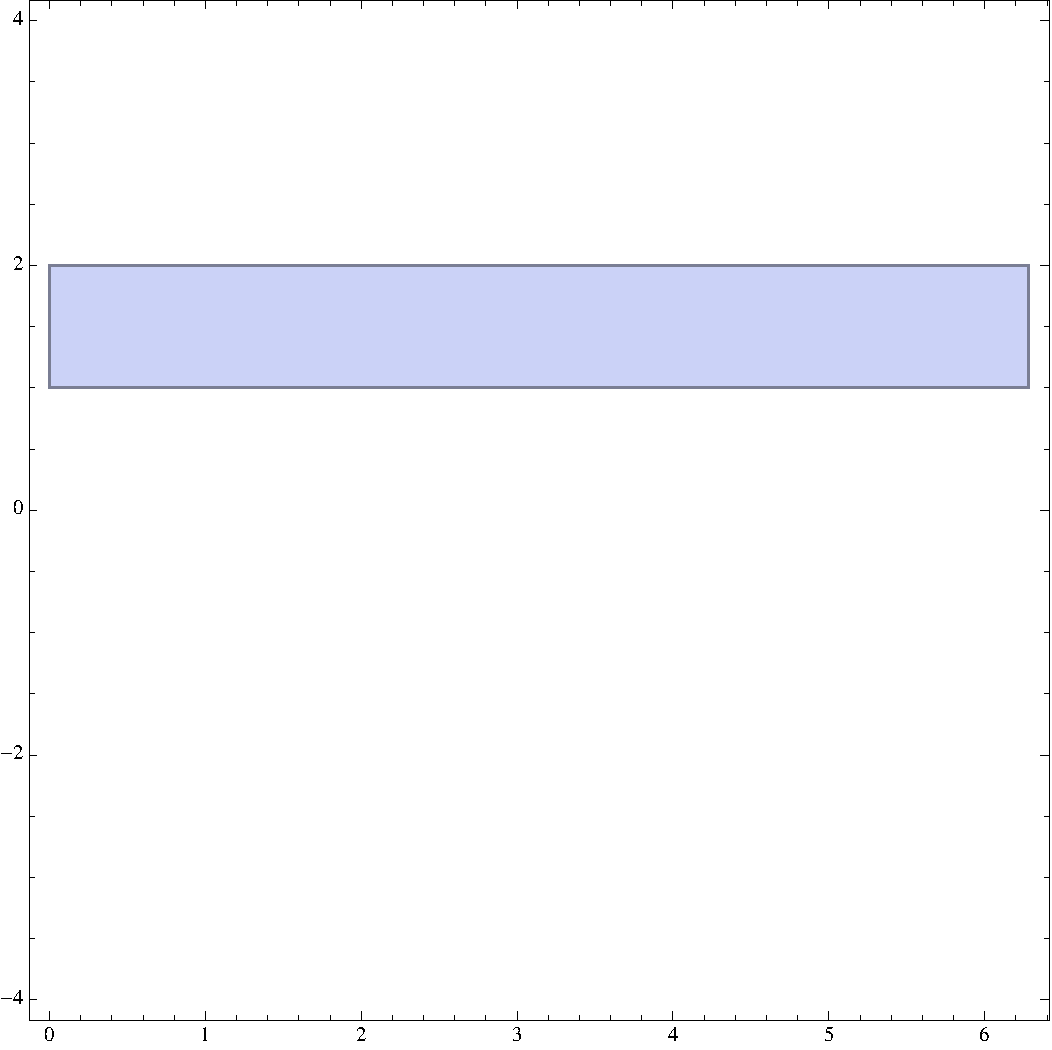
\includegraphics[width=5cm]{./figures/2.3-2.5/pic2.pdf}
\caption{A quantum state in phase space}
\end{figure}\\
Since the angle $\varphi$ varies between $0$ and $2\pi$, angular momentum should be quantized as shown:
$$
h = 2\pi\Delta L\quad \Rightarrow \quad \Delta L =\hbar
$$
Since we starting from the zero line, the eigenvalues of energy should be
\begin{equation}
E_m = f(m\hbar)
\end{equation}
Notice that we get this result by cutting the phase space into slices without solving the Schr$\ddot{\mathrm{o}}$dinger Equation. Because the Hamiltonian commutes with the angular momentum, the eigenenergy is given by eigenvalues of the angular momentum:
$$
-i\hbar \frac{\partial \psi}{\partial\varphi} = L\psi\quad\psi(\varphi) =\psi(\varphi+2\pi)
$$
solve the differential equation and the result is:
$$
L = m\hbar\quad m \in \mathbb{Z}\,.
$$
Now we find that the result we get from the eigenfunction of angular momentum operator is the same as we get from cutting the phase space into cells.


\section*{Problem 2.4}
If we just consider about the orbital angular momentum, it can be written as a function of $p_\theta$ and $p_\varphi$ which are the canonical momentum conjugate to the spherical coordinate variables $\theta$ and $\varphi$: 
\begin{equation}
L^2 = p_\theta^2 + \frac{p_\varphi^2}{\sin^2 \theta}
\end{equation}
thus the phase volume of the region which satisfies $L^2 \leq M^2$ is
\begin{eqnarray}
\bf{\Omega}& = &\int_0^\pi d\theta \int_0^{2\pi} d\varphi \int_{L^2\leq M^2} dp_\theta dp_\varphi\nonumber\\
&=& \int_0^\pi d\theta \int_0^{2\pi} d\varphi \, \pi  M^2\sin\theta\nonumber\\
&=& 4\pi^2 M^2
\end{eqnarray}
Thus the number of microstates is $\Omega = {\bf{\Omega}}/h^2 = M^2/\hbar^2$. Then let us calculate the number by quantized angular momentum. By summing up all the eigenstates of the angular momentum, we get:
\begin{equation}
\Omega = \sum_{j=0}^{j_{\mathrm{max}}}(2j+1) = (j_{\mathrm{max}}+1)^2
\end{equation}
Now we have to determine the number $j_{\mathrm{max}}$. Since we want the absolute value of the angular momentum $ \sqrt{j_{\mathrm{max}}(j_{\mathrm{max}}+1)}\hbar< M$, we can find that $j_{\mathrm{max}}$ is determined by the following equation:
\begin{equation}
j_{\mathrm{max}} = \Big{\lfloor} \frac{\sqrt{1+\frac{4M^2}{\hbar^2}}-1}{2}\Big{\rfloor}
\end{equation}
It is obvious that $j_\mathrm{max} = \lfloor M/\hbar\rfloor -1$ or $j_\mathrm{max} = \lfloor M/\hbar\rfloor$. So the total number of microstates will be:
\begin{equation}
\Omega = \Big{\lfloor} \frac{M}{\hbar}\Big{\rfloor}^2\,\mathrm{or}\,\left(\Big{\lfloor} \frac{M}{\hbar}\Big{\rfloor}+1\right)^2
\end{equation}
If we take the classical limit that $M \gg \hbar$, the result will be:
\begin{equation}
\Omega \simeq \frac{M^2}{\hbar^2}
\end{equation}


\section*{Problem 2.5}
In this problem we need to use the WKB approximation in Quantum Mechanics. 
\begin{figure}[!htp]
\centering
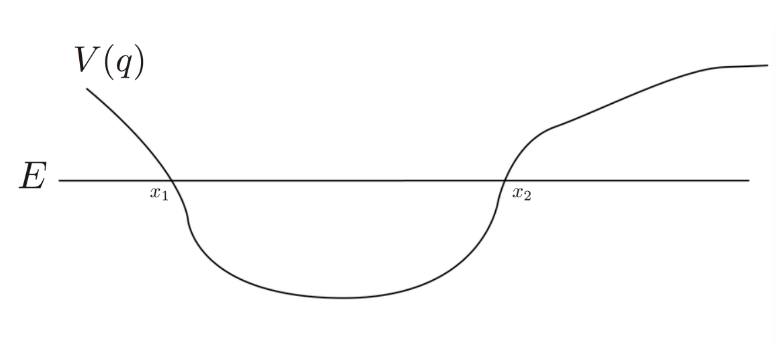
\includegraphics[width=10cm]{./figures/2.3-2.5/pic1.png}
\caption{WKB Approximation}
\end{figure}
In D. Griffiths' book we find that the WKB wave function between two classical turning point $x_1$ and $x_2$ is:
$$
\psi(x) = \frac{2D}{\sqrt{p(x)}}\sin\left[\frac{1}{\hbar}\int_x^{x_2}p(x')dx' + \frac{\pi}{4}\right]\quad\quad x< x_2
$$
or
$$
\psi(x) = -\frac{2D'}{\sqrt{p(x)}}\sin\left[-\frac{1}{\hbar}\int_{x_1}^{x}p(x')dx'-\frac{\pi}{4}\right]\quad\quad x>x_1
$$
in which $p(x) = \sqrt{2m[E-V(x')]}$. We can define:
\begin{eqnarray*}
\theta_1(x) &=& \frac{1}{\hbar}\int_{x_1}^{x}p(x')dx'+\frac{\pi}{4}\\
\theta_2(x) &=& \frac{1}{\hbar}\int_x^{x_2}p(x')dx' + \frac{\pi}{4}
\end{eqnarray*}
Since the two solutions should be the same, the difference between the two $\theta$ functions should be $n\pi, n\in\mathbb{Z}$: 
\begin{equation}
n\pi-\frac{\pi}{2} = \frac{1}{\hbar}\int_{x_1}^{x_2}p(x')dx'
\end{equation}
The integral in classical phase space is
$$
\oint p\,dq = 2 \int_{x_1}^{x_2}p(x')dx'
$$
so finally we can find that 
\begin{equation}
\oint p\,dq = h\left(n-\frac{1}{2}\right)\quad n\in\mathbb{Z}\,.
\end{equation}
\section*{Problem 2.6}
The equation of phase space orbit is:
$$
\frac{1}{2}ml^{2}\dot{\theta}^{2}+\frac{1}{2}mgl\theta^{2}=E
$$
This is a eclipse whose area is:
$$
S=\pi \sqrt{2Eml^{2}}\sqrt{\frac{2E}{mgl}}=2\pi E \sqrt{\frac{l}{g}}=E \tau
$$
\section*{Problem 2.7}
\subparagraph{(i)}
Assume that these N SHOs are distinguishable.To distribute total energy E into such N SHOs,\quad there are 
$$C_{E/\hbar \omega+N/2-1}^{N-1}$$ways. \quad 
Let\quad $E/\hbar \omega >>N$ ,we get the approximate result: 
$$
\frac{1}{(N-1)!} (\frac{E}{\hbar \omega} )^{N-1}
$$
\subparagraph{(ii)}
The total energy of N classical SHOs is:
$$\sum_{i=1}^{N}(\frac{p_i^2}{2m}+\frac{k x_i ^2}{2})=E$$
The phase space volume is:
$$(\frac{2}{\omega})^N E^{N-1} \pi ^N \frac{1}{(N-1)!} dE$$
while dE=$\hbar \omega$,\quad we get\quad $\omega_0=h^N$

\end{document}
